\newpage
\setcounter{page}{1}
\justifying
\noindent

\section{Introduction}
\subsection{Formula Student}
Formula student United Kingdom (FSUK) is an annual motor-sport engineering competition held by Institute of Mechanical Engineers (IMechE). Every July since 2007, hundreds of universities from around the world gather at Silverstone Circuit for the final competition. Every team's objective is to design and build a single-seat race car, which will be judged from several engineering and business aspects. The competition mainly consists of two events: static and dynamics. The static event judges the Engineering  Design,  Cost and  Sustainability  Analysis, Business Presentation and Technical Inspection, and the dynamic event evaluates Skid Pad, Sprint, Acceleration, Endurance, and Fuel.

\begin{figure}[!ht]
\begin{center}
%    
  \begin{subfigure}[b]{0.45\textwidth}
    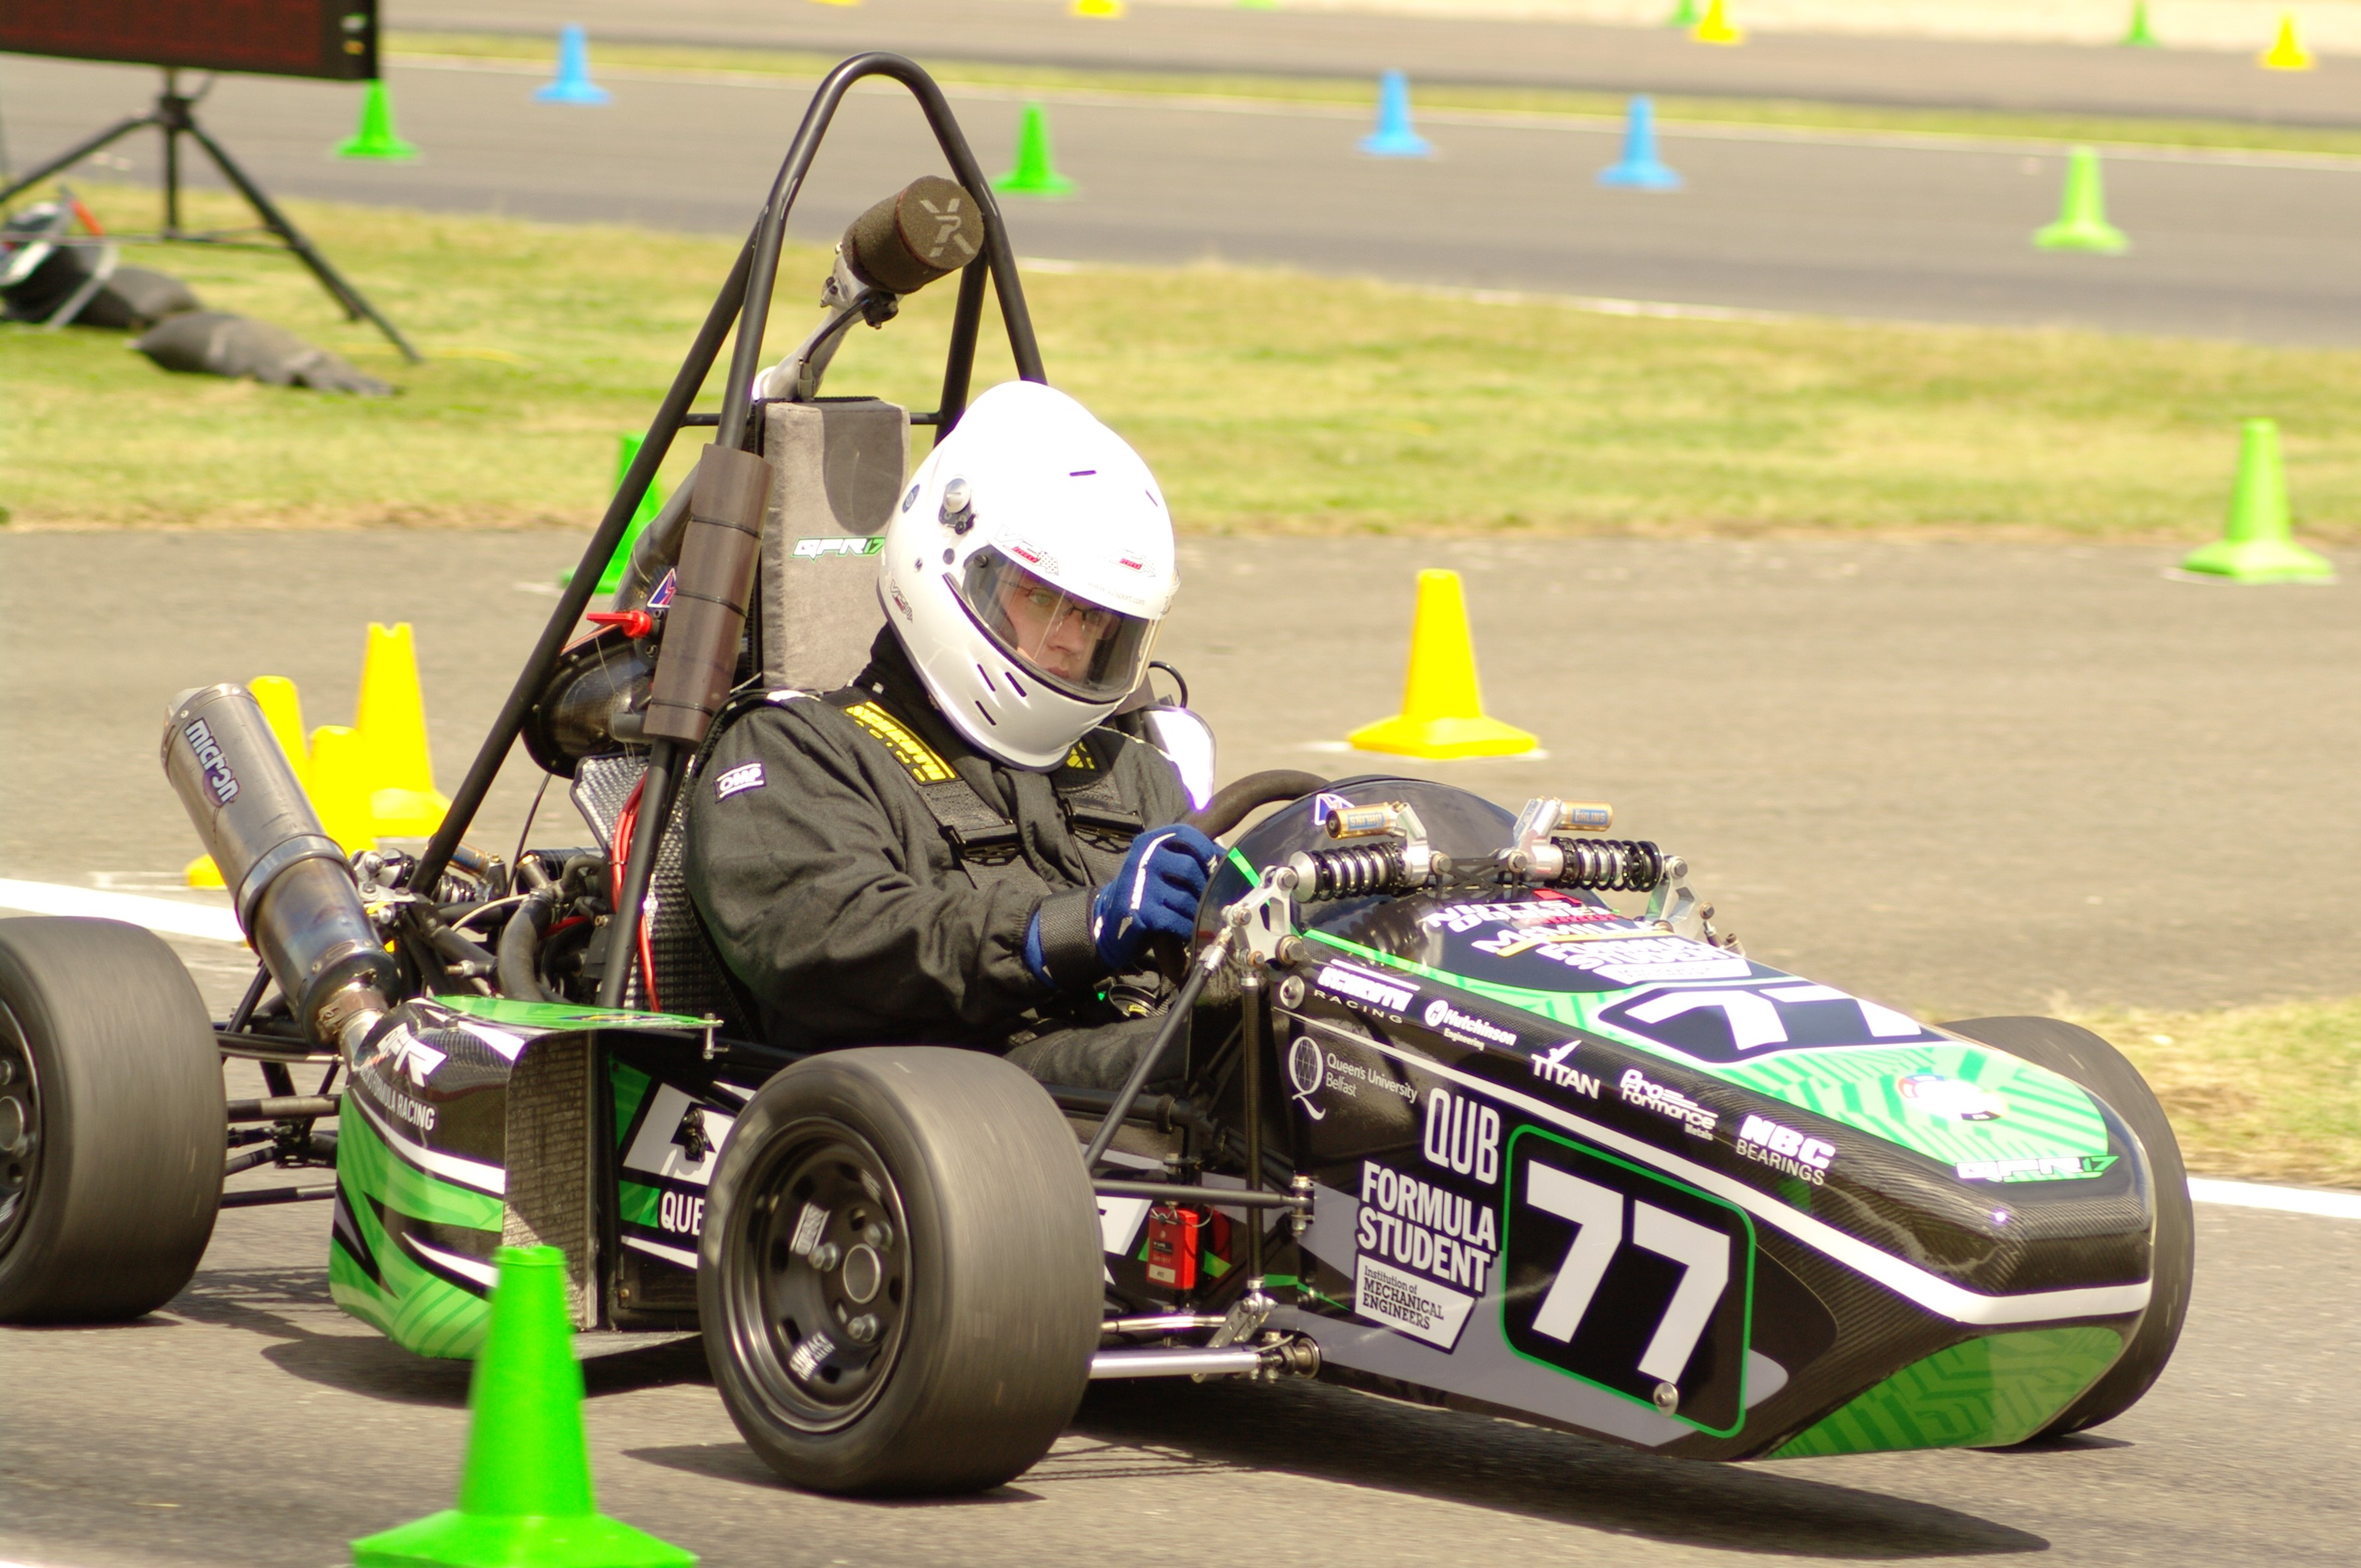
\includegraphics[height=4.5cm]{Figures/QFR17PHOTO.JPG}
  \end{subfigure}
  %
  \begin{subfigure}[b]{0.45\textwidth}
    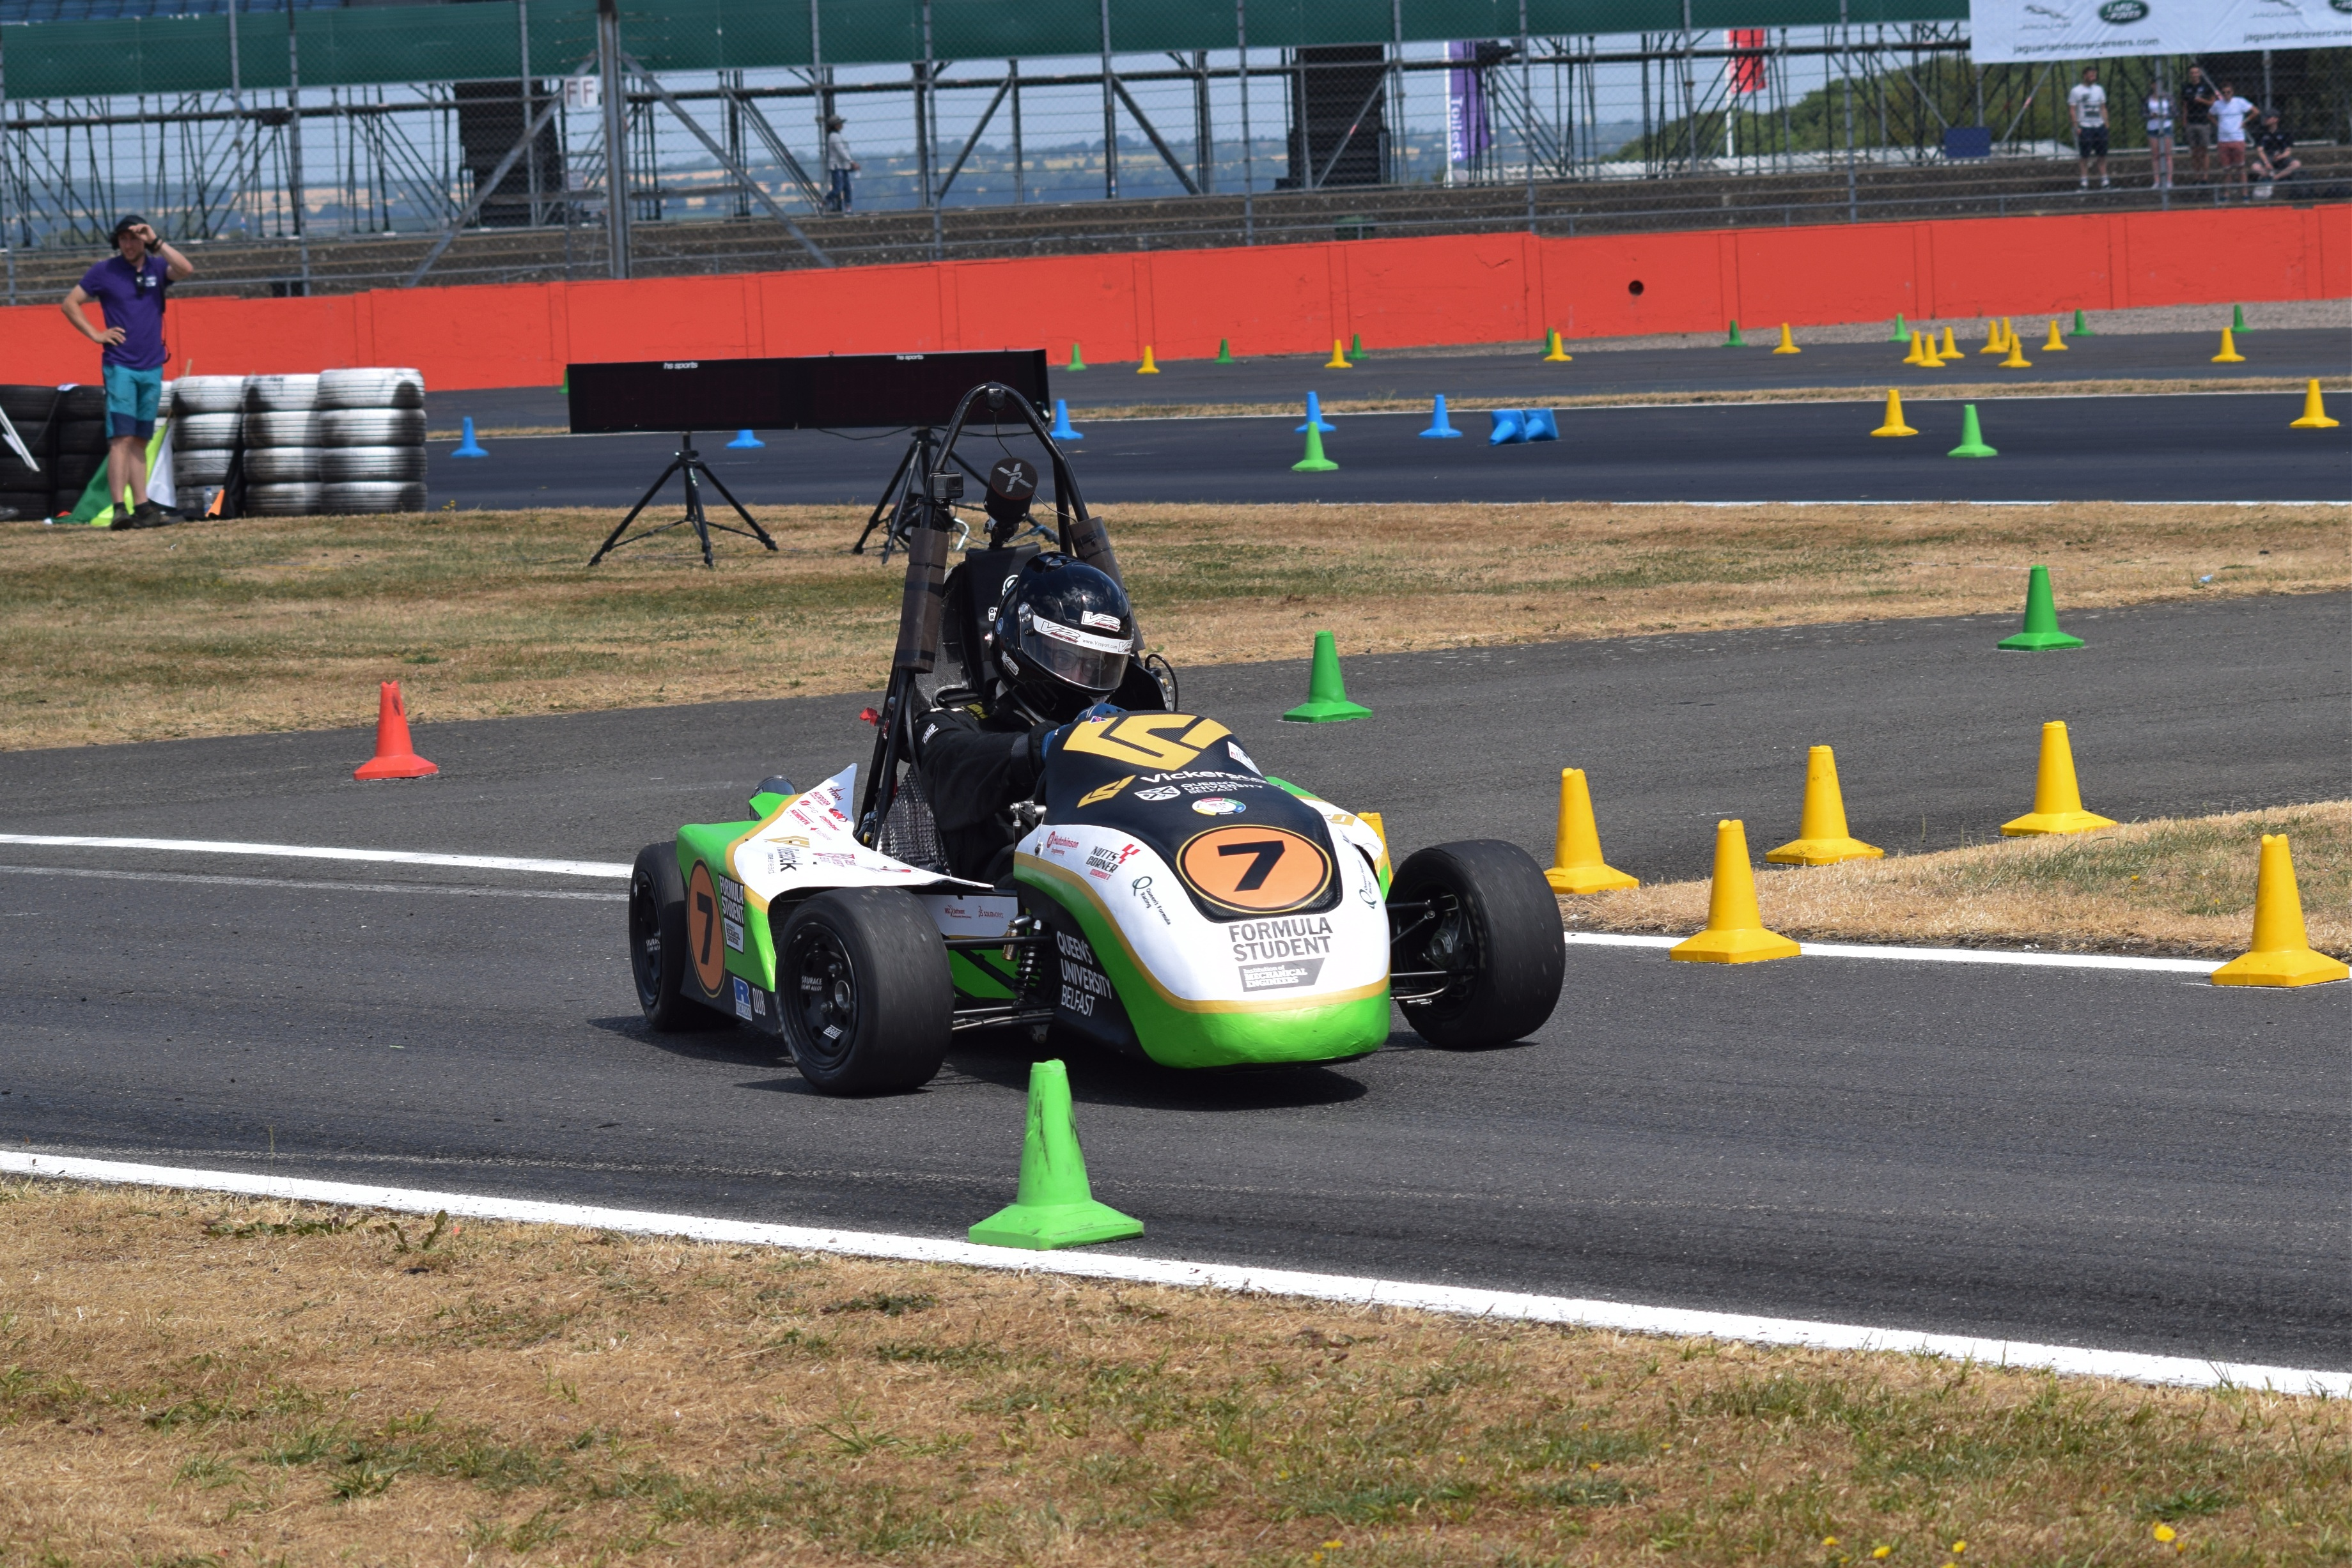
\includegraphics[height=4.5cm]{Figures/QFR18PHOTO.jpg}
  \end{subfigure}
%  
  \caption{Queen's Formula Racing car 2017 (left) and 2018 (right) on the dynamics event}
    \label{fig:1}
\end{center}
\end{figure}

\noindent Queen's Formula Student first initiated consideration of aerodynamic aspects on QFR car in 2017, which focus on the aerodynamic analysis framework \cite{Corr2017MechanicalAuthor}. In 2018 the first design of aerodynamics undertray for QFR race car was generated \cite{McKeown2018DesignCar}. This paper is intended to build up the analyses from previous papers and improve the undertray performance by investigating broader and deeper variables that could plausibly enhance the overall car performance. 

\subsection{The significance of Aerodynamics in Formula Industry}
Aerodynamics has become a crucial aspect of high-speed cars performance. The race-car industry has led the technology innovation by indicating the needs for constant improvements \cite{Zhang2006GroundCars}. Engineers have been striving to sculpt the car's shape to manipulate and advantage the body's flow. The role of aerodynamics in improving the race-car performance rose in 1968 when inverted airfoil was introduced to Formula One car, and the research in this area has been growing exponentially ever since. 

%put inverted aerofoil race car photo here

\noindent Downforce(negative-lift) is a significant aerodynamics key in improving the overall race car's performance. Downforce or negative lift is the force product of the aerodynamics flow around the body. This is usually achieved on a high-speed ground vehicle by introducing aerodynamic devices such as wing (inverted wing) and undertray, which modify the airflow to the engineering needs \cite{Wright1982TheCars}. In the race-car industry, the primary aim is to maximise the downforce while maintaining the drag at the lowest \cite{Zhang2006GroundCars}, but achieving consistent performance at diverse speed and acceleration is equally essential.  The size of the downforce is significantly affected the breaking acceleration and cornering, hence the cornering speed. Despite the restrictive aerodynamics rules in the competition, optimising the downforce could improve the acceleration, increasing the chance to overturn the opponent on a corner. Higher downforce could also increase the top speed in a shorter time, reducing the corner entry and exit time. 

\noindent However, A ground-effect aerodynamics that applied to an open-wheeled car is still an experimental science \cite{Zhang2006GroundCars}, this is due to the complex physics flow that involves turbulent wake, the interaction of ground boundary layer, dynamic suspension motion, and many more in which accurate analytical capability (experimental \& computational) is not yet sufficient.

\noindent Nevertheless, computational fluid dynamics (CFD) has improved tremendously with the industry over the years and produced accurate results of forces, flow pattern, etc., in some particular car geometry. However, one research paper \cite{Zhang2006GroundCars} stated that race car diffuser is one of the most complex parts which hardly to be understood. Therefore specific variable in generating an undertray geometry is required with careful consideration and assumption on the analysis. 

\noindent This paper will utilise CFD to understand the trend behaviour of an aerodynamics undertray in 2 dimensions and three dimensions with several nozzle \& diffuser variables such as angle, length, and width. These results will then be used to consider the geometry dimension of the final aerodynamics undertray for QFR 2021.

\subsection{Project Aims \& Objectives}
This project aims to design and optimise the aerodynamics undertray for Queen's Formula Racing car, which improve the car's overall down-force and drag reduction. The undertray's final design will be based on the computational simulations and design recommendation from previous QFR analysis. The approved final design then will be manufactured and installed to QFR 2021 for the competition if the workshop time and capacity allows.

\noindent
Some objectives were made to fulfil the aim:
\begin{itemize}

    \item Analyse the enclosed and open flow 2D \& 3D analyses with various inlet, outlet, and ground clearance variables using ANSYS Fluent to identify its effect and trend on the undertray lift and drag. 
    
    \item Design flexible 3D undertray designs based on the 2D analysis results, which will again be optimised with additional aerodynamic features on the undertray, improving the downforce and reducing the drag.
    
	\item Design the final undertray CAD and choose the material which tailored to the car’s dimension and goals, then analyse the weight to drag ratio to pick the best performance and material for the car.
	
    \item Manufacture and fit the undertray for 2021 Queen’s Formula Racing car, which then will be judged on the Formula Student competition.
\end{itemize}